%% W dokumencie nie określono podstawowych parametrów!
%% Nie polecam korzystać z niego jako podstawy od budowy swoich prezentacji ;)

\documentclass[
  size=14pt,
  mode=present,
  paper=a4paper,
  clock,
  style=sailor
]{powerdot}			%%określenie klasy dokumentu jako

\usepackage{polski}
\usepackage[utf8]{inputenc}

\title{Zadanie 003 -- PowerDot}
\author{Krystian Oleniacz}
\date{11.10.2018 r.}

\begin{document}					%%począetk dokumentu
\maketitle

\begin{slide}{spis treści}
	\tableofcontents[content=sections]
\end{slide}

\section[toc={Zadania}]{Sekcja Zadania do wykonania}



\begin{slide}{Odtworzenie prezentacji}
	Państwa zadaniem jest stworzenie prezentacji, które będzie zawierać treści i wyglądać identycznie jak ta prezentacja. \pause
	
	W katalogu znajdują się potrzezbne pliki graficzne.	
\end{slide}


\section{Sekcja Druga}
\begin{slide}{Spis treści sekcji 2}
	\tableofcontents[content=currentsection]
	\end{slide}
\begin{slide}{Dwie kolumny 1}
	\twocolumn[lcolwidth=0.7\linewidth, rcolwidth=0.2\linewidth]{Dwie kolumny?
		Kolumna o szerokości 0,7 szerokości
		lini}{Kolumna prawa o szerokości 0,2 szekorości linii}
	
	
	
	
	A jakże! - tekst pod dwiema kolumnami
\end{slide}

\begin{slide}{Dwie kolumny 2}
	Dwie kolumny z grafikami?
	\twocolumn[lcolwidth=0.47\linewidth, rcolwidth=0.47\linewidth]
	{\centering
		 $h=3h$
		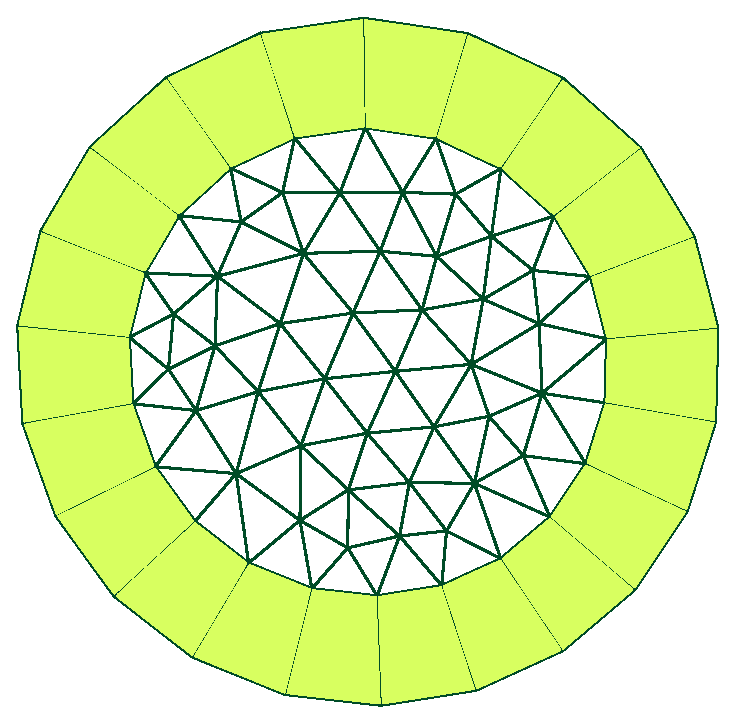
\includegraphics[width=1.0\linewidth]
		{fig_onsolving3d_penny_mesh.eps}
	$N = 86?$}
	{\centering $h=3h^*$
		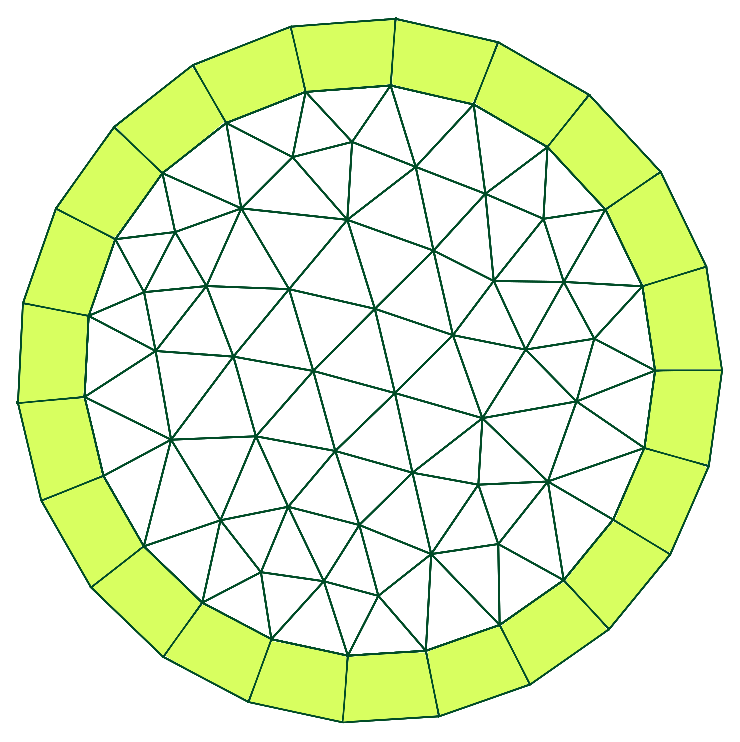
\includegraphics[width=1.0\linewidth]
		{fig_onsolving3d_penny_mesh_2.eps}
	$N=86?$}
	

A jakże! - grafika w dwóch kolumnach
\end{slide}	

\section[tocsection=hidden]{Sekcja A - Brak w spisie treści, widoczna po lewej gdy aktywna sekcja wcześniejsza}
\begin{slide}{Slajd 3}
3	
\end{slide}	
\section{Sekcja A - czasem widać, czasem nie widać :}
\begin{slide}{Slajd 4}
4	
\end{slide}

\section{Sekcja bez pozycji w spisie}
\begin{slide}{Slajd 5}
5	
\end{slide}	

\begin{slide}{Slajd 6}
6
\end{slide}	

\section{Grafika 2}

\begin{slide}{Kolejny slajd będzie bez tytułu slajdu, ale z grafiką}
	\centering
	Wycinek walca:\\
	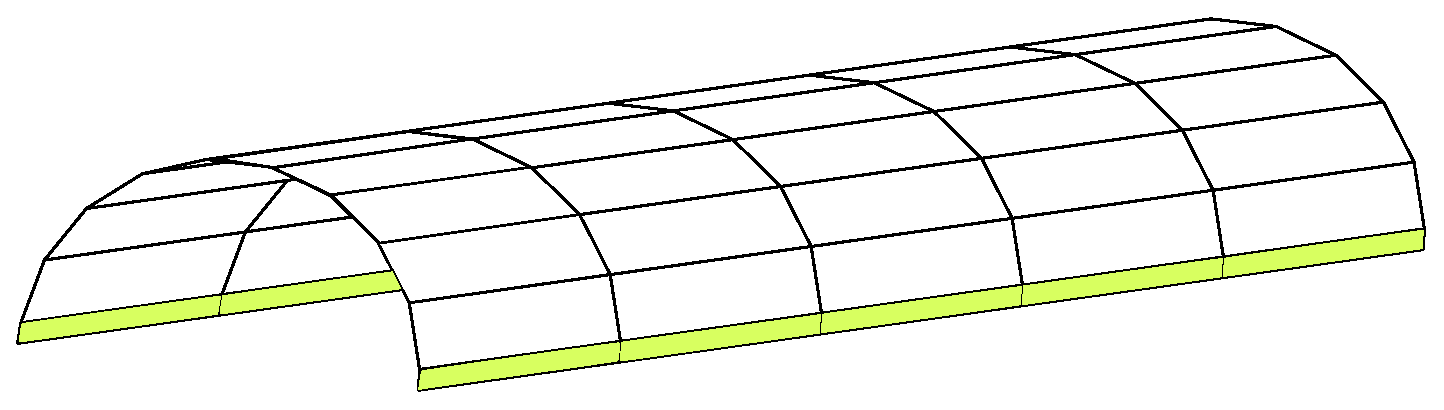
\includegraphics[width=0.75\slidewidth]{fig_onsolving3d_cylinder.eps}

\end{slide}

\begin{emptyslide}{pusty 1}
	\centering
	\vspace{\stretch{1}}
	Jego przekrój
	
	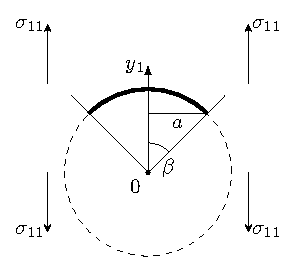
\includegraphics[height=0.6\slideheight]
	{fig_onsolving3d_crosssection_cylindrical.eps}
	\vspace{\stretch{1}}
\end{emptyslide}

\begin{emptyslide}{pusty 2}
	\centering
	\vspace{\stretch{1}}
	Koniec!
	
	
\includegraphics[height=0.6\slideheight]{fig_onsolving3d_blocks.eps}
	\vspace{\stretch{1}}
	
\end{emptyslide}


\end{document}						%%koniec dokumentu